\documentclass[a4paper, 12pt]{article}

\usepackage{babel}
\usepackage{enumitem}
\usepackage{times}
\usepackage{graphicx}
\usepackage{geometry}
	\geometry{left = 4cm, top = 4cm, right = 3cm, bottom = 3cm}
\usepackage{float}
\usepackage{setspace}
	\setstretch{1.5}
\usepackage{listings}


\begin{document}
\title{\huge\textbf{Tugas Praktikum Pemrograman II (Chapter 4)}}
\date{}

\maketitle


\begin{figure}[!ht]
\begin{center}

\includegraphics[width = 6cm, height = 6cm]{poltekpos.jpg}
\end{center}
\end{figure}

\begin{center}
\vspace{1cm}
Disusun oleh :\\
Putri Nella\\
D4 TI 2C\\
1.18.4.017\\
\vspace{1cm}
\textbf{PROGRAM DIPLOMA IV POLITEKNIK POS INDONESIA} \linebreak
\textbf{POLITEKNIK POS INDONESIA} \linebreak
\textbf{BANDUNG}\linebreak
\textbf{2019}

\end{center}


\thispagestyle{empty}

\chapter{Pengelolaan File CSV}

Tujuan pembelajaran pada pertemuan keempat antara lain:
\begin{enumerate}
\item
Mengenal file CSV dan fungsinya 
\item
Mengerti cara memakai library CSV
\item
Mengerti cara memakai library pandas
\item
Mengatasi Error yang terjadi akibat pemakaian library csv dan pandas
\item
Try Except
\end{enumerate}
Tugas dengan cara dikumpulkan dengan pull request ke github dengan menggunakan latex pada repo yang dibuat oleh asisten IRC. Kode program dipisah dalam folder src NPM.py yang berisi praktek dari masing-masing tugas file terpisah sesuai nomor yang kemudian dipanggil menggunakan input listing ke dalam file latex penjelasan atau nomor pengerjaan. Masing masing soal bernilai 5 dengan total nilai 100. Gunakan bahasa yang baku dan bebas plagiat dengan dibuktikan hasil scan plagiarisme. Serta hasil scrinsut dari komputer sendiri, dan kode hasil sendiri. Pengerjaan menggunakan latex dan harus menyertakan file pdf hasil compile pdflatex, jika tidak diskon 50\%.


\section{Pemahaman Teori}
Kerjakan soal berikut ini, masing masing bernilai 5. Untuk hari pertama.
Praktek teori penunjang yang dikerjakan dengan deadline besok jam 4 pagi:
\begin{enumerate}
\item
Apa itu fungsi file csv, jelaskan sejarah dan contoh
\item
Aplikasi-aplikasi apa saja yang bisa menciptakan file csv?
\item
Jelaskan bagaimana cara menulis dan membaca file csv di excel atau spreadsheet
\item
Jelaskan sejarah library csv
\item
Jelaskan sejarah library pandas
\item
Jelaskan fungsi-fungsi yang terdapat di library csv
\item
Jelaskan fungsi-fungsi yang terdapat di library pandas
\end{enumerate}

\section{Ketrampilan Pemrograman}
Kerjakan soal berikut ini, masing masing bernilai 5 untuk hari kedua, lusa jam 4 pagi. Soalnya adalah:

\begin{enumerate}
\item
Buatlah fungsi (file terpisah/library dengan nama NPM\_csv.py) untuk membuka file csv dengan lib csv mode list
\item
Buatlah fungsi (file terpisah/library dengan nama NPM\_csv.py) untuk membuka file csv dengan lib csv mode dictionary
\item
Buatlah fungsi (file terpisah/library dengan nama NPM\_pandas.py) untuk membuka file csv dengan lib pandas mode list
\item
Buatlah fungsi (file terpisah/library dengan nama NPM\_pandas.py) untuk membuka file csv dengan lib pandas mode dictionary
\item
Buat fungsi baru di NPM\_pandas.py untuk mengubah format tanggal menjadi standar dataframe
\item
Buat fungsi baru di NPM\_pandas.py untuk mengubah index kolom
\item
Buat fungsi baru di NPM\_pandas.py untuk mengubah atribut atau nama kolom
\item
Buat program main.py yang menggunakan library NPM\_csv.py yang membuat dan membaca file csv
\item
Buat program main2.py yang menggunakan library NPM\_pandas.py yang membuat dan membaca file csv
\end{enumerate}




\section{Ketrampilan Penanganan Error}
Kerjakan soal berikut ini, masing masing bernilai 5(hari kedua). Bagian Penanganan error dari script python.
\begin{enumerate}
\item
Tuliskan peringatan error yang didapat dari mengerjakan praktek ketiga ini, dan jelaskan cara penanganan error tersebut.
dan Buatlah satu fungsi yang menggunakan gunakan try except untuk menanggulangi error tersebut.
\end{enumerate}



\section{Presentasi Tugas}
Pada pertemuan ini, diadakan dua penilaiain yaitu penilaian untuk tugas mingguan seperti sebelumnya dengan nilai maksimal 100. Kemudian dalam satu minggu kedepan maksimal sebelum waktu mata kuliah kecerdasan buatan. Ada presentasi kematerian dengan nilai presentasi yang terpisah masing-masing 100. Jadi ada tiga komponen penilaiain pada pertemuan ini yaitu :
\begin{enumerate}
	\item tugas minggu hari ini dan besok (maks 100). pada chapter ini
	\item presentasi csv (maks 100). Mempraktekkan kode python dan menjelaskan cara kerjanya.
\end{enumerate}
Waktu presentasi pada jam kerja di IRC. Kriteria penilaian presentasi sangat sederhana, presenter akan ditanyai 20(10 pertanyaan program, 10 pertanyaan teori) pertanyaan tentang pemahamannya menggunakan python untuk kecerdasan buatan. jika presenter tidak bisa menjawab satu pertanyaan asisten maka nilai nol. Jika semua pertanyaan bisa dijawab maka nilai 100. Presentasi bisa diulang apabila gagal, sampai bisa mendapatkan nilai 100 dalam waktu satu minggu kedepan.





\section{PEMAHAMAN TEORI}
\begin{enumerate}
\item Apa itu fungsi file csv, jelaskan sejarah dan contoh
\subsection{Fungsi file CSV}
fungsi  Comman Separated Value (CSV) yaitu sebagai format data yang akan memudahkan penggunanya untuk melakukan penginputan data ke database secara sederhana. CSV juga bisa digunakan dalam standar file ASCII, di mana pada setiap record dipisahkan dengan tanda koma (,) atau titik koma (;).\\ sejarah csv Inisiatif standardisasi utama — mentransformasikan "definisi fuzzy de facto " menjadi definisi yang lebih tepat dan de jure - adalah pada tahun 2005, dengan RFC4180, mendefinisikan CSV sebagai Tipe Konten MIME . Kemudian, pada 2013, beberapa kekurangan RFC4180 ditangani oleh rekomendasi W3C.\\
Ketika user menerima file dengan format CSV, yang biasanya bertuliskan .CSV, maka file tersebut akan terbuka dalam format Microsoft Excel.
\subsection{Sejarah}
	IBM Fortran (level H extended) compiler di bawah OS/360 mendukung fomat CSV pada tahun 1972. FORTRAN 77 mendefinisikan penulisannya dimana input atau output yang menggunakan tanda koma atau spasi untuk pembatas antara data dan penulisan tersebut sudah disetujui pada tahun 1978.
\\	Osborne Executive computer yang mengembangkan SuperCalc       spreadsheet pada tahun 1983 membuat konvensi kutipan CSV      yang memungkinkan string mengandung koma(,).
\\
	Inisiatif standardisasi utama \- mentransformasi \"definisi fuzzy defacto\" menjadi definisi yang lebih tepat dan de jure \-adalah pada tahun 2005, dengan RFC4180, mendefinisikan CSV sebagai Tipe Konten MIME. Kemudian, pada tahun 2013, beberapa kekurangan RFC4180 ditangani oleh rekomendasi W3C.
\\
	Pada 2014 IETF menerbitkan RFC7111 yang menjelaskan aplikasi fragmen URI pada dokumen CSV. RFC7111 menentukan bagaimana rentang baris, kolom, dan sel dapat dipilih dari dokumen CSV menggunakan indeks posisi.
\\
	Pada 2015 W3C, dalam upaya meningkatkan CSV dengan semantik formal, mempublikasikan draftrekomendasi pertama untuk stadar metadata CSV, yang dimulai sebagai rekomendasi pada bulan Desembertahun yang sama.

\item Aplikasi-aplikasi apa saja yang bisa menciptakan suatu file dalam bentuk csv
\begin{enumerate}
\item Editor Text (Sublime, Notepad, Atom, visual studio code dan lain-lain) 
\item Spreadshett (Microsoft Excel, google spreadsheet,libreOfficecalc dan lain-lain)
\end{enumerate}
\item Jelaskan bagaimana cara menulis dan membaca file csv di excel atau spreadsheet
\begin{enumerate}
\subsection{Menulis File CSV}
\item Pertama-tama kita buka terlebih dahulu aplikasi microsoft excel, dengan cara klik start dan cari excel kemudian enter
\item Kemudian setelah aplikasi microsoft excel terbuka lalu kita klik Blank Workbokk

\item Setelah Blank Workbook terbuka lalu kita tulis sesuai data yang diinginkan 
 
\item Setelah data selesai dibuat maka save file tersebut dengan cara klik file lalu save as dan piih browse
 
\item Lalu kita beri nama data filenya pada File Name dan ubah type file pada Save as type menjadi .csv
 
\item Kemudian kita klik save
 
\item Kemudian file yang telah dibuat tadi tersimpan dengan ekstensi .csv. Dan untuk melihat isi filenya tinggal klik dua kali pada file tersebut.

\item Ini adalah isi file yang telah dibuat

\subsection{Untuk melihat File CSV di Excel atau Spreadsheet}
\item Pertama kita klik dua kali pada file yang yang berekstensi CSV.
	
\item Setelah itu file akan terbuka secara otomatis di aplikasi Excel atau spreadsheet.
\end{enumerate} 
\item Sejarah library csv
\\
Library csv mengimplementasikan kelas yang digunakan untuk membaca dan menulis data dalam format csv. Ini memungkinkan seorang programmer untuk mengatakan "baca data dari file ini yang dihasilkan oleh Excel". Pemrogram juga bisa menentukan format csv sesuai dengan keinginan mereka sendiri.
\item sejarah library pandas
\\
Pengembangan pandas dimulai pada tahun 2008 di AQR Captal Management. Pandas pada akhir 2009 telah menjadi open source dan secara aktif didukung oleh komunitas individu yang berpikiran sama dengan seluruh indonesia yang menyumbangkan waktu dan energi mereka untuk membuat sebuah pandas yang bersifat open source. 
\\
Pandas adalah sebuah proyek yang di sponsori oleh NumFOCUS sejak 2005. Ini akan sangat membantu untuk memastikan sebuah keberhasilan pengembangan pandas sebagai sebuah proyek sumber terbuka kelas dunia.
\item Jelaskan fungsi-fungsi yang terdapat di library csv
\begin{enumerate}
\item reader
\hfill\break
	Reader memiliki fungsi yang digunakan untuk membaca isi file yang berformat CSV dari list.
    
\item DictReader
\hfill\break
	DictReader memiliki fungsi yang digunakan untuk membaca isi file yang berformat CSV dari dictionary.
	
\item write
\hfill\break
	Write memiliki fungsi yang digunakan untuk menulis pada suatu file yang berformat CSV dari list.
	
\item DictWrite
\hfill\break
	DictWrite juga memiliki fungsi yang digunakan untuk menulis file yang berformat CSV dari dictionary.

\end{enumerate}
\item Jelaskan fungsi-fungsi yang terdapat di library pandas
\begin{enumerate}
\item read\_csv
\hfill\break
	Fungsi ini digunakan untuk membaca isi file berformat CSV

\item to\_csv
\hfill\break
	Fungsi ini digunakan untuk menulis file berformat CSV

\end{enumerate}
\section{Bukti bebas Plagiarism}
\begin{figure}[H]
			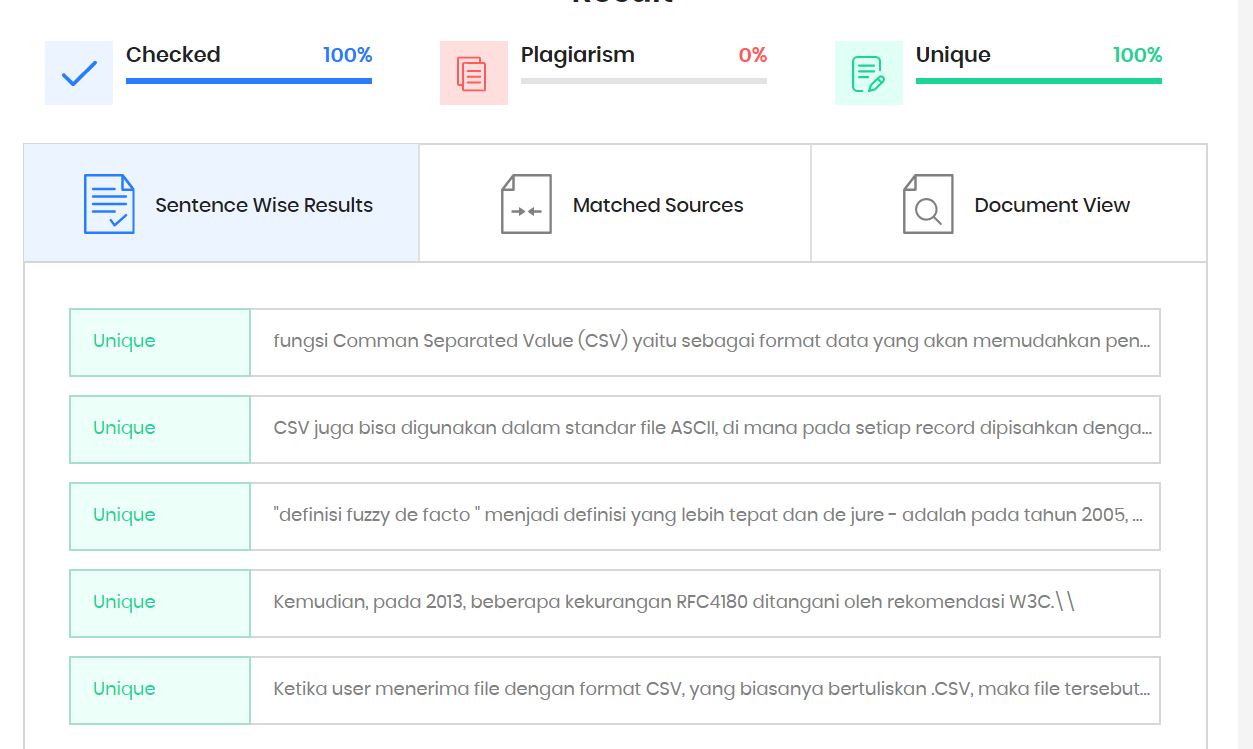
\includegraphics[width=8cm]{figure/1.PNG}
			\centering
			\caption{Bukti Screenshot bebas plagiarism}
	\end{figure}
\section{Ketrampilan Pemrogaman}
\begin{enumerate}
\item Buatlah fungsi (file terpisah/library dengan NPM\_csv.py) untuk membuka file csv dengan lib csv mode list.

\item Buatlah fungsi (file terpisah/library dengan nama NPM\_csv.py) untuk membuka file csv dengan lib csv mode dictionary

\item Buatlah fungsi (file terpisah/library dengan nama NPM\_pandas.py) untuk membuka file csv dengan lib pandas mode list

\item Buatlah fungsi (file terpisah/library dengan nama NPM\_pandas.py) untuk membuka file csv dengan lib pandas mode dictionary
\item Buat fungsi baru di NPM\_pandas.py untuk mengubah format tanggal menjadi standar dataframe
\item Buat fungsi baru di NPM\_pandas.py untuk mengubah index kolom
\item Buat fungsi baru di NPM\_pandas.py untuk mengubah atribut atau nama kolom
\item Buat program main.py yang menggunakan library NPM\_csv.py yang membuat dan membaca file csv

\item Buat program main2.py yang menggunakan library NPM\_pandas.py yang membuat dan membaca file csv

\end{enumerate}
\section{Bukti bebas Plagiarism}
\begin{figure}[H]
			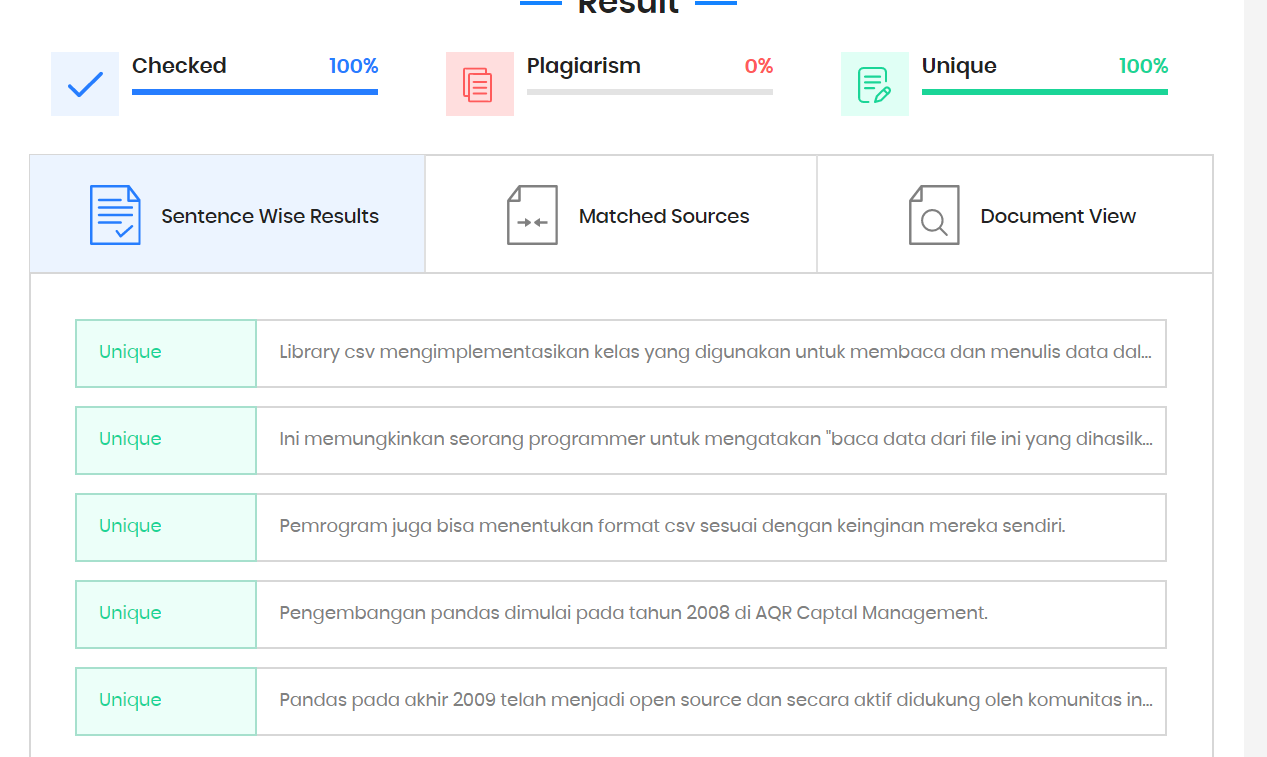
\includegraphics[width=8cm]{figure/2.PNG}
			\centering
			\caption{Bukti Screenshot bebas plagiarism}
	\end{figure}
\end{enumerate}

\end{document}
